\chapter{Feature List}
\section{Einleitung}
In diesem Kapitel werden \textit{Features} beschrieben, die im Rahmen dieser Arbeit implementiert werden können.
Für alle \textit{Features} wird der Nutzen beschrieben und auch mögliche Probleme identifiziert.
Die \textit{Features} werden in Teilziele unterteilt und nach Nutzen und geschätztem Arbeitsaufwand bewertet.
Am Schluss werden alle Teilziele nach dem besten Nutzen-Aufwand Verhältnis sortiert, um die die \textit{Features} zu identifizieren, welche sich am meisten zu implementieren lohnen.


\section{Essential Features}
\subsection{Beschreibung}
\textit{Essential Features} sind alle Features, welche von allen anderen Features benötigt werden und grundsätzlich notwendig sind, um EEROS mit ROS zu verwenden.


\section{Daten über einen ROS-Knoten empfangen}
\subsection{Beschreibung}
Eine EEROS-Applikation soll Daten von diversen Quellen über einen ROS-Knoten empfangen können.
Mögliche Quellen sind Sensoren (Microsoft Kinect) oder Steuerungsbefehle.
Die Steuerungsbefehle sollen über eine GUI, eine Tastatur oder einen XBox-Controller\footnote{siehe dazu 'joy'\_packet http://wiki.ros.org/joy} gesendet werden können.


\section{Logging (Protokollierung)}
\subsection{Beschreibung}
Mit \textit{Logging} sind Ausgaben gemeint, die den aktuellen Status der EEROS-Applikation wiedergeben.
Sie können auch für Fehlermeldungen und Debug-Informationen verwendet werden.

Das EEROS-Framework hat bereits eine Logger-Funktionalität.
In der aktuellen EEROS-Version kann der \textit{Loggers}  mit folgenden Zeilen benutzt werden\footnote{http://wiki.eeros.org/tools/logger/start?s[]=log}:
\lstset{language=C++}
\begin{lstlisting}
StreamLogWriter w(std::cout); Logger log(); log.set(w);
log.info() << "Logger Test";
int a = 298;
logg.warn() << "a = " << a;
log.error() << "first line" << endl << "second line"; 
\end{lstlisting}

In EEROS erfolgt die Ausgabe des \textit{Loggers} über die Konsole (\textit{StreamLogWriter}) oder in eine Datei (\textit{SysLogWriter}).
Wenn die Ausgabe auf einem anderen PC erfolgen soll, z.B. bei einem ferngesteuerten Roboter, kann eine SSH-Verbindung hergestellt werden.

EEROS bietet auch eine Möglichkeit um Informationen im \textit{Control System} zu loggen\footnote{http://wiki.eeros.org/tools/logger\_cs/start}.
Dabei stellt sich das Problem, dass das \textit{Control System} normalerweise sehr oft (1000 Mal in der Sekunde) ausgeführt wird und den Bildschirm mit Informationen überfluten würde.
Es existiert aber bereits eine Lösung mit \textit{Periodic Functions}, damit die Daten mit einer viel kleineren Frequenz ausgegeben werden.
Die Lösung mit den \textit{Periodic Functions} ist aber nicht intuitiv und wird oft, besonders in der Debugging-Phase nicht genutzt und umgangen.

ROS hat mit der \textit{ROS console}\footnote{http://wiki.ros.org/rosconsole} eine ausgereifte Logging-Funktion integriert.
Mit der \textit{Throttle-Funktion} (\texttt{ROS\_DEBUG\_THROTTLE(period, ...)} bietet ROS eine sehr bequeme Möglichkeit, um eine Information nur einmal in einem bestimmten Zeitraum auszugeben.
Weitere Funktionen sind noch:

\begin{itemize}
\item ROS\_DEBUG\_COND(cond, ...)
\item ROS\_DEBUG\_ONCE(...)
\item ROS\_DEBUG\_DELAYED\_THROTTLE(period, ...)
\item ROS\_DEBUG\_FILTER(filter, ...)
\end{itemize}

Wie auch EEROS hat ROS verschiedene \textit{verbosity levels} um Debug-Informationen von normalen Informationen, Warnungen und Fehlern zu unterscheiden.

Ein weiterer Vorteil bei ROS ist, dass die Ausgaben irgendwo im ROS-Netzwerk, also auch auf einem anderen PC, gelesen und in eine Datei gespeichert werden können.
Zusätzlich existieren schon ausgereifte Programme, welche die Ausgaben live filtern, farblich hervorheben und ausgeben können.
\textit{rqt\_console} ist ein solches Programm, dass auch schon standardmässig mit ROS installiert wird.
In Bild \ref{fig:rqtConsole} ist ein Screenshot von \textit{rqt\_console} zu sehen.

\begin{figure}[!ht]
\centering
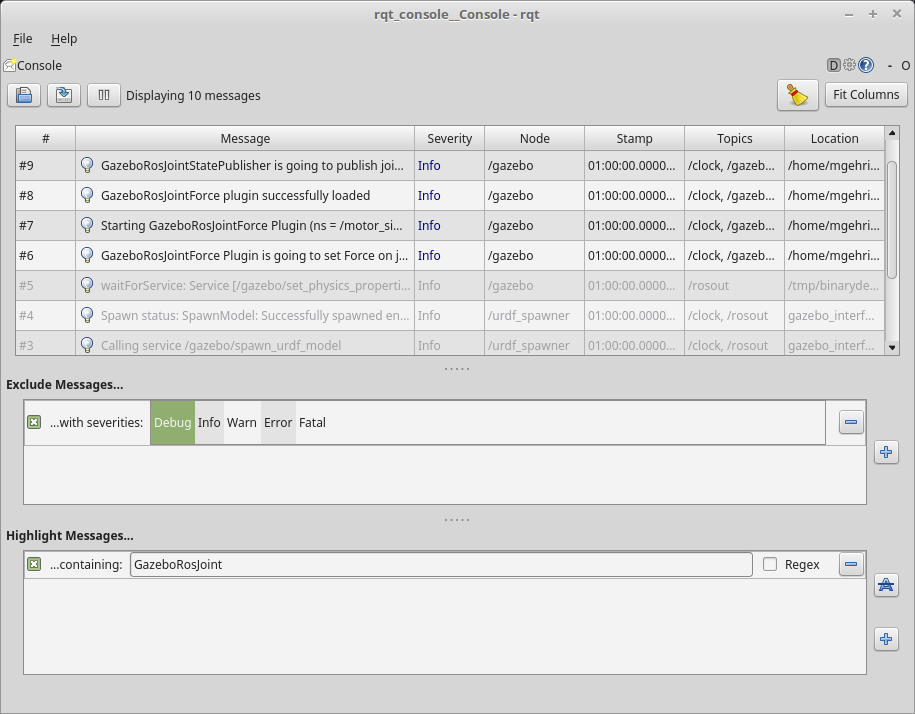
\includegraphics[angle=0,width=\textwidth]{images/screenshotRqtConsole.png}
\caption{\textit{rqt\_console} ist ein ROS-Tool, um Log-Nachrichten darzustellen und zu filtern}
\label{fig:rqtConsole}
\end{figure}


\section{Anzeige von Prozessvariablen}
\subsection{Beschreibung}
Prozessvariablen sind, im Gegensatz zu den Log-Ausgaben, einzelne Zahlen oder Datenpunkte wie beispielsweise die Position eines Encoders.
Die Variablen können in einem GUI angezeigt werden.
Im einfachsten Fall zeigt das GUI die Variablen in einer einfachen Konsole an.
In vielen Fällen ist es aber von Vorteil, wenn eine oder mehrere Variablen in einem Graphen visualisiert werden können.

\subsection{Zu erwartende Probleme}
Bei Prozessvariablen gilt es zu beachten, dass sehr schnell eine grosse Menge von Daten anfallen können.
Dabei ist nicht nur die Bandbreite ein Problem, sondern auch die Latenz.
Im konkreten Fall bedeutet dies, dass in einem \textit{Control System} bei jedem Durchlauf innerhalb von sehr kurzer Zeit (typischerweise \unit[1]{msec}) neue Daten produziert werden.
Wenn das ROS-Netzwerk nicht innerhalb einer Millisekunde die Daten wegschicken kann, kann es sein, dass Daten verloren gehen.

Eine Lösung für die zu geringe Latenz des ROS-Netzwerks wäre ein Buffer, der den hochfrequenten Datenstrom abfängt und in längeren Zeitabständen (etwa \unit[0.1]{s} bis \unit[1]{s}) Datenpakete mit den Daten schickt.

%TODO auf performance messungen verweisen dei zeigen, dass das kein problem is

Wenn aber die Bandbreite zu hoch ist, das heisst, wenn mehr Daten durch das ROS-Netzwerk geschickt werden, als das Netzwerk übertragen kann, dann reicht ein einfacher Buffer nicht mehr aus.
Folgende Techniken könnten das Problem lösen:
\begin{itemize}
\item \textbf{Throttle:} Funktioniert wie der Logger mit \textit{Throttle}-Funktionalität. Die meisten Daten werden verworfen und nur jeder x-te Wert wird geschickt.
\item \textbf{Zeitbegrenzter Buffer:} Ein Buffer speichert über eine begrenzte Zeit die Daten und schickt sie dann mit reduzierter Bandbreite über das Netzwerk.
\item \textbf{Filter:} Es werden nur Daten gesendet, die eine bestimmte Bedingung erfüllen. Z.B. wenn deren Wert grösser als 10 ist.
\item \textbf{Statistik:} Für eine gewisse Anzahl von Datenpunkten werden statistische Werte, wie z.B. Mittelwert, Minimum und Maximum berechnet. Dem Netzwerk werden nur die berechneten Werte gesendet.
\end{itemize}


\section{Simulation mit Gazebo}
\subsection{Beschreibung}
\textit{Gazebo} ist eine Simulationssoftware für Roboter.
Wenn der physikalische Roboter von \textit{Gazebo} simuliert wird, dann kann die EEROS-Applikation getestet werden, ohne dass die Hardware vorhanden sein muss.
Nachdem die Applikation und die Regelung mit der Simulation getestet und verfeinert wurde, kann sie auf dem Richtigen Roboter getestet werden.

Idealerweise wird wird dafür die HAL von EEROS genutzt.
So muss nur die Konfigurationsdatei der HAL angepasst werden, wenn von der Simulation zur richtigen Hardware gewechselt wird.

\subsection{Zu erwartende Probleme}
Eine Simulation muss nicht in Echtzeit erfolgen.
Wenn es eine komplexere Simulation ist, oder wenn die Simulation visualisiert werden soll, dann ist der Rechner oft zu langsam, um die Simulation in Echtzeit zu rechnen.
Die Kommunikation mit ROS ist ebenfalls nicht echtzeitfähig.

Eine Simulation von einem dynamischen System ist aber stark abhängig von der Zeit.
Es muss also sicher gestellt werden, das die Simulation und auch die EEROS-Applikation mit der richtigen Zeit rechnet, damit auch Regler getestet werden können.
Zusätzlich muss sicher gestellt werden, dass die Simulation und die Applikation abwechselnd rechnen, um \textit{Race Conditions} zu vermeiden.


\section{Bewertung der verschiedenen Features und Teilziele}
\subsection{Beschreibung des Punktesystems}
In Tabelle \ref{Bewertungstabelle} werden alle oben genannten Features werden in Teilziele aufgeteilt und deren Nutzen und Aufwand mit einem Wert zwischen 0 und 10 bewertet.
Die Punkte für jedes Teilziel werden berechnet, in dem der Nutzen durch den Aufwand dividiert wird.
Mit dieser Methode sollen diejenigen Teilziele gefunden werden, die mit möglichst kleinem Aufwand einen möglichst grossen Nutzen bringen..

In der Tabelle \ref{BewertungstabelleSortiert} sind alle Teilziele nach dem Punktewert sortiert.
Nur die \textit{Essential Features} bilden eine Ausnahme, da sie von allen anderen Features benötigt werden.
Deshalb sind sie an erster Stelle.

Alle Features werden dann der Reihe nach implementiert.
Sollte im Rahmen dieser Arbeit nicht genügend Zeit vorhanden sein um alle Teilziele zu implementieren, dann werden die Teilziele ganz unten, also die mit dem schlechtesten Nutzen-Aufwand Verhältnis, nicht implementiert.


\subsection{Bewertungstabelle}
\label{Bewertungstabelle}
\begin{tabular}
  { l								| l			 								l			 l			 l }
  \textbf{Feature}					& \textbf{Teilziel}	& \textbf{Nutzen}	& \textbf{Aufwand}	& \textbf{Punkte}	\\ \hline
  
% Feature							  Teilziel   								Nutzen      Aufwand     Punkte
  Essential							& 1. Unabhängiger ROS-Knoten				& 10		& 3			& 3.3		\\
  									& 2. CMAKE									& 10		& 4			& 2.5		\\ \hline
  Daten empfangen					& 1. Einfacher ROS-Knoten					& 8			& 3			& 2.7		\\
  									& 2. Generischer ROS-Knoten					& 8			& 4			& 2.0		\\
  									& 3. HAL									& 8			& 7			& 1.1		\\
  									& 4. Generischer Tastaturknoten				& 7			& 5			& 1.4		\\ 
  									& 4. XBox-Controller						& 7			& 5			& 1.4		\\ \hline
  Daten senden						& 1. Konsolenausgabe 						& 8			& 5			& 1.6		\\
  									& 2. Diagramm								& 8			& 6			& 1.3		\\
  									& 3. Gazebo									& 10		& 8			& 1.3		\\
  									& 4. Throttle-Funktion						& 8			& 6			& 1.3		\\
  									& 5. Zeitbegrenzter Buffer					& 6			& 6			& 1.0		\\
  									& 6. Filter									& 6			& 6			& 1.0		\\
  									& 7. Statistik								& 7			& 7			& 1.0		\\ \hline
  Logging 							& 1. EEROS-Logger umlenken					& 4			& 4			& 1.0		\\
  									& 2. \textit{Verbosity levels} beibehalten	& 2			& 5			& 0.4		\\
  									& 3. \textit{Throttle}-Funktionalität		& 4			& 6			& 0.7		\\
  									& 4. \textit{Conditional}-Funktionalität 	& 3			& 3			& 1.0		\\
  									& 5. \textit{Once}-Funktionalität			& 3			& 3			& 1.0		\\
  									& 6. \textit{Filter}-Funktionalität			& 1			& 3			& 0.3		\\
  									& 7. \textit{Delayed-Throttle}-Funkt.		& 1			& 3			& 0.3		\\ \hline
%  Manipulieren von Prozessvar.		& 1. Ausgänge setzen						& 8			& 4			& 2.0		\\
%  									& 2. Konstanten setzen						& 6			& 4			& 1.5		\\ \hline
  Simulation mit Gazebo				& 1. Einfacher PI Regler					& 8			& 5			& 1.6		\\
  									& 2. Korrekter Zeitstempel und Sync.		& 9			& 6			& 1.5		\\ \hline
\end{tabular}

\subsection{Bewertungstabelle sortiert}
\label{BewertungstabelleSortiert}
\begin{tabular}
  { l								| l			 								l			 l			 l 		l}
  \textbf{Feature}					& \textbf{Teilziel}	& \textbf{Nutzen}	& \textbf{Aufwand}	& \textbf{Punkte}	& \textbf{Impl.}	\\ \hline
  
% Feature							  Teilziel   							Nutzen      Aufwand     Punkte
  Essential							& Unabhängiger ROS-Knoten				& 10		& 3			& 3.3	&\cmark	\\
  Essential							& CMAKE									& 10		& 4			& 2.5	&\cmark	\\ 
  Daten empfangen					& Einfacher ROS-Knoten					& 8			& 3			& 2.7	&\cmark	\\
  Daten empfangen					& Generischer ROS-Knoten				& 8			& 4			& 2.0	&\cmark	\\
  Daten senden						& Konsolenausgabe 						& 8			& 5			& 1.6	&\cmark	\\
  Simulation mit Gazebo				& Einfacher PI Regler					& 8			& 5			& 1.6	&\cmark	\\ 
  Simulation mit Gazebo				& Korrekter Zeitstempel und Sync.		& 9			& 6			& 1.5	&\cmark	\\
  Daten empfangen					& Generischer Tastaturknoten			& 7			& 5			& 1.4	&\cmark	\\ 
  Daten empfangen					& XBox-Controller						& 7			& 5			& 1.4	&\xmark	\\ 
  Daten senden						& Diagramm								& 8			& 6			& 1.3	&\cmark	\\
  Daten senden						& Gazebo								& 10		& 8			& 1.3	&\cmark	\\
  Daten senden						& Throttle-Funktion						& 8			& 6			& 1.3	&\xmark	\\
  Daten empfangen					& HAL									& 8			& 7			& 1.1	&\cmark	\\
  Daten senden						& Zeitbegrenzter Buffer					& 6			& 6			& 1.0	&\xmark	\\
  Daten senden						& Filter								& 6			& 6			& 1.0	&\xmark	\\
  Daten senden						& Statistik								& 7			& 7			& 1.0	&\xmark	\\ 
  Logging 							& EEROS-Logger umlenken					& 4			& 4			& 1.0	&\xmark	\\
  Logging							& \textit{Conditional}-Funktionalität 	& 3			& 3			& 1.0	&\xmark	\\
  Logging							& \textit{Once}-Funktionalität			& 3			& 3			& 1.0	&\xmark	\\
  Logging							& \textit{Throttle}-Funktionalität		& 4			& 6			& 0.7	&\xmark	\\
  Logging							& \textit{Verbosity levels} beibehalten	& 2			& 5			& 0.4	&\xmark	\\
  Logging							& \textit{Filter}-Funktionalität		& 1			& 3			& 0.3	&\xmark	\\
  Logging							& \textit{Delayed-Throttle}-Funkt.		& 1			& 3			& 0.3	&\xmark	\\ 
%  Manipulieren von Prozessvar.		& Ausgänge setzen						& 8			& 4			& 2.0	&\xmark	\\
%  Manipulieren von Prozessvar.		& Konstanten setzen						& 6			& 4			& 1.5	&\xmark	\\ 
\end{tabular}